\documentclass[12pt,a4paper]{article}
\usepackage[utf8]{inputenc}
\usepackage{graphicx}
\usepackage{hyperref}
\usepackage{geometry}
\usepackage{float}
\usepackage{listings}
\usepackage{xcolor}

\geometry{a4paper, margin=2cm}

\title{\textbf{Laporan Praktikum: Implementasi CRUD Mahasiswa dengan Flask dan MySQL}}
\author{
    \textbf{Fransiscus Asisi Kananda Herdion Dharmawan} \\
    NIM: 24.83.1107 \\
    Teknik Komputer \\
    Universitas Amikom Yogyakarta
}
\date{\today}

\begin{document}

\maketitle

\section{Informasi Proyek}
Laporan ini disusun untuk memenuhi tugas praktikum implementasi CRUD (Create, Read, Update, Delete) menggunakan *framework* web Python, Flask, yang diintegrasikan dengan *database* relasional MySQL. Seluruh dokumentasi dan *source code* dari proyek ini telah diunggah ke repositori GitHub publik.

\textbf{Tautan Repositori GitHub Proyek:} \\
\url{https://github.com/diondharmawan/Amikom-Tugas-Flask-CRUD}

\section{Implementasi Sistem}
Sistem Informasi Manajemen Data Mahasiswa ini dibuat dengan arsitektur sederhana di mana Flask bertindak sebagai *backend* yang merespons permintaan HTTP, dan Jinja2 bertindak sebagai *template engine* untuk merender halaman HTML. Desain antarmuka menggunakan **AdminLTE** dan **Bootstrap** untuk memberikan tampilan yang profesional dan responsif. Basis data menggunakan MySQL dengan nama basis data \texttt{db\_kuliah} dan tabel \texttt{mahasiswa}.

\section{Dokumentasi Source Code dan Eksekusi}
Berikut adalah dokumentasi hasil eksekusi program beserta cuplikan kode.

\begin{figure}[H]
    \centering
    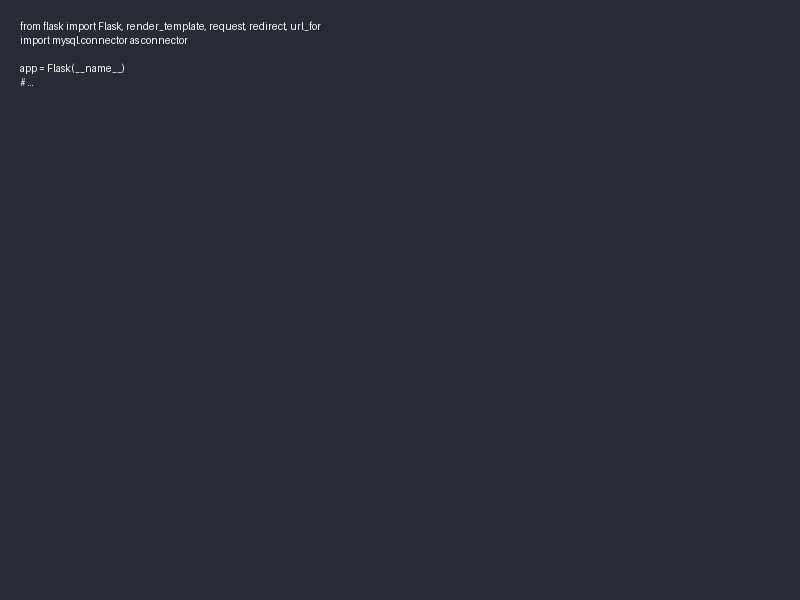
\includegraphics[width=0.9\textwidth]{sc_code.png}
    \caption{Cuplikan Source Code Utama (\texttt{app.py})}
    \label{fig:sccode}
\end{figure}

\begin{figure}[H]
    \centering
    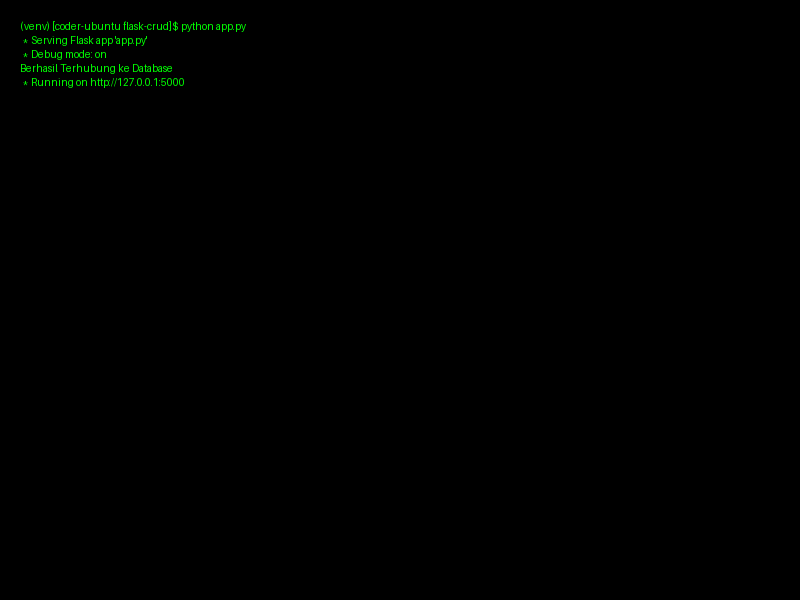
\includegraphics[width=0.9\textwidth]{sc_output.png}
    \caption{Output Terminal saat Eksekusi Flask}
    \label{fig:scoutput}
\end{figure}

\begin{figure}[H]
    \centering
    
\includegraphics[width=0.9\textwidth]{sc_crud_index.png}
    \caption{Tampilan Halaman Utama (Read Data)}
    \label{fig:scindex}
\end{figure}

\begin{figure}[H]
    \centering
    
\includegraphics[width=0.9\textwidth]{sc_crud_tambah.png}
    \caption{Tampilan Form Tambah Data (Create Data)}
    \label{fig:sctambah}
\end{figure}

\begin{figure}[H]
    \centering
    
\includegraphics[width=0.9\textwidth]{sc_crud_ubah.png}
    \caption{Tampilan Form Ubah Data (Update Data)}
    \label{fig:scubah}
\end{figure}

\section{Kesimpulan}
Implementasi CRUD menggunakan Flask dan MySQL berjalan dengan lancar. Penggunaan \texttt{mysql-connector-python} mempermudah komunikasi antara aplikasi web dan sistem manajemen basis data. Selain itu, dengan penerapan *templating* menggunakan Jinja2, antarmuka AdminLTE dapat digunakan ulang pada berbagai halaman (menggunakan fitur \texttt{\{\% extends 'base.html' \%\}}) sehingga kode HTML menjadi lebih terstruktur, modular, dan mudah dikelola.

\end{document}
